The framework we provide utilizes the advantages of the Python and Javascript 
programming languages. Python has been proven to be efficient for data analysis 
tasks, and Javascript is designed to enable interactive actions for browser-based 
applications. A customizable Python script and template file are used to generate 
a static HTML page with associated resources (Javascript, CSS, and images) to 
display the browser-based user interface. The static page can be shared with 
collaborators over email or file exchange without requiring the setup of a web 
server. The results of a researcher's analysis are saved in the browser using 
the HTML5 Storage API, and can be exported as CSV files. The framework is 
flexible and expandable to incorporate new data analysis algorithms and 
visualization methods. In addition to the framework, we also provide three 
implementations for analyzing ambiguous crowd-sourced labels, outlier detection 
and correction, and dynamic classification error analysis.

\begin{figure}
	\centering
	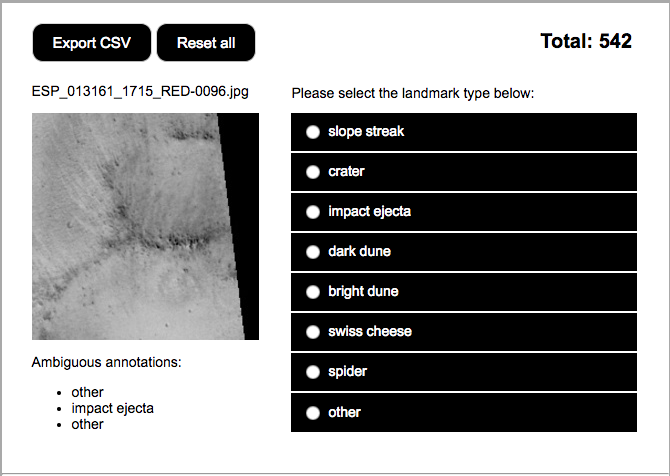
\includegraphics[width=3in]{images/ala-ui}
	\caption{Ambiguous Label Analyzer}
	\label{fig:ala}
\end{figure}


\subsection{Ambiguous Label Analyzer}
Crowd-source labeling is an efficient method to collect a huge amount of labeled 
data for machine learning system. The Ambiguous Label Analyzer, as shown in 
Figure \ref{fig:ala}, is created for generating consensus labels by taking the 
majority vote. If there is no majority vote, the image is categorized as ambiguous, 
which will be further reviewed and assigned a label by domain experts.  

\begin{figure}
        \centering
        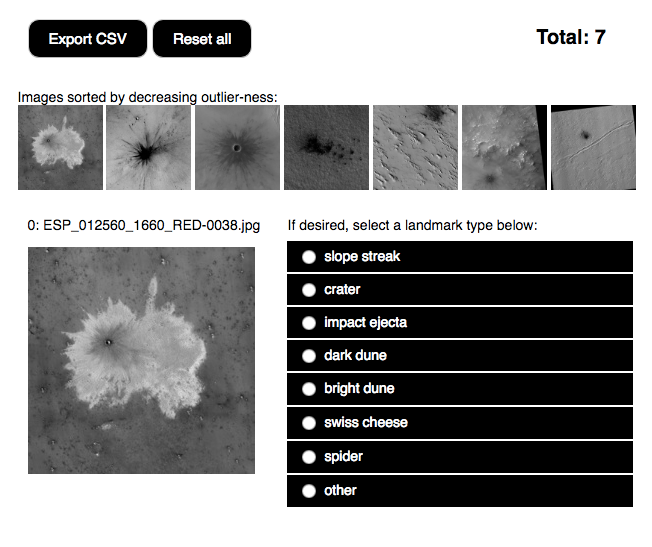
\includegraphics[width=3in]{images/oia-ui}
        \caption{Outlier Analyzer}
        \label{fig:oia}
\end{figure}


\subsection{Outlier Analyzer}
One method for identifying mislabeled items within a data set is to find outliers 
within each class and check to see if they should instead be assigned to a 
different class. The Outlier Analyzer, as shown in Figure \ref{fig:oia}, is 
created to estimate images' outlier-ness using singular-value decomposition (SVD) 
reconstruction error. The image with the highest SVD reconstruction error is 
considered to be an outlier, and options are provided to re-assign the label 
for the outlier. 

\begin{figure}
        \centering
        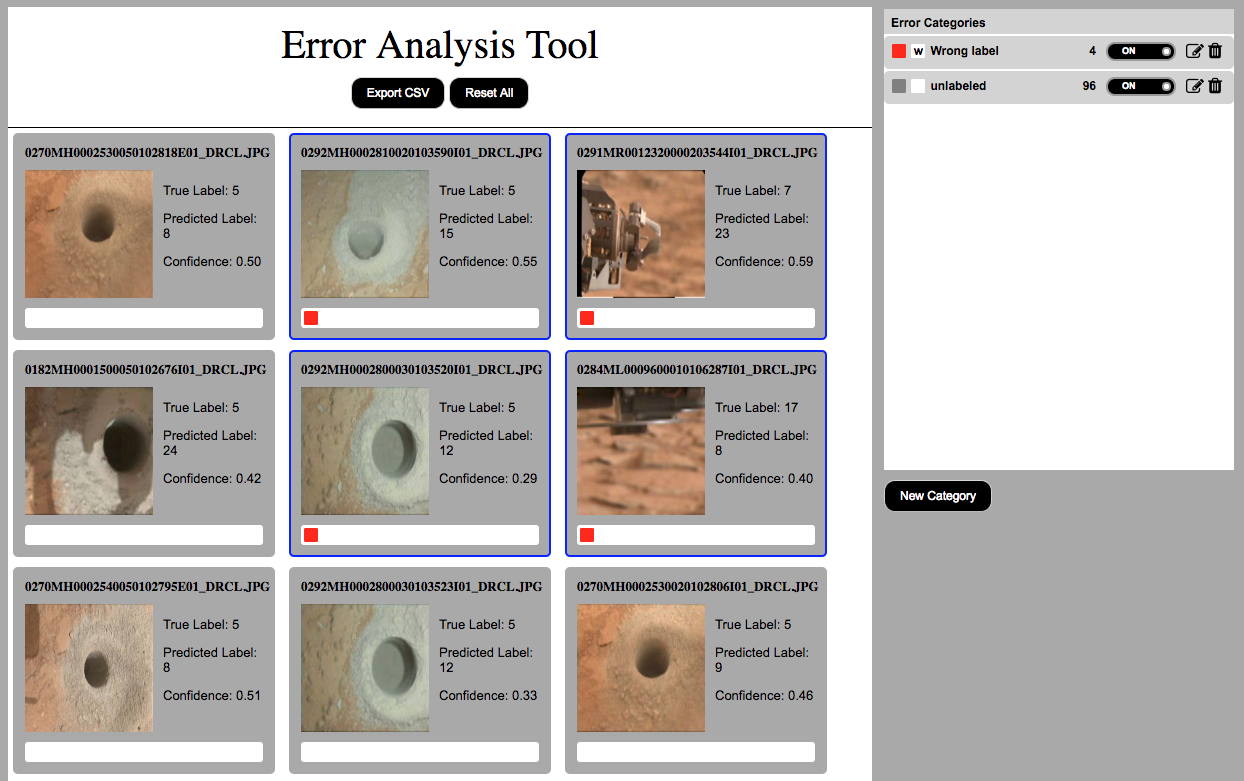
\includegraphics[width=3.4in]{images/eat-ui}
        \caption{Classification Error Analyzer}
        \label{fig:eat}
\end{figure}

\subsection{Classification Error Analyzer}
Studying the classification errors made by a machine learning system is an 
important step to iteratively improve the model's performance. The Classification 
Error Analyzer, as shown in Figure \ref{fig:eat}, is a tool that provides the 
capability of conducting interactive and dynamic error analysis. Each image 
displayed on the left side of the web page will be tagged with one or more error 
categories shown on the right side of the web page. New error categories can be 
created dynamically. The corrective actions will be taken to fix the most common 
errors, and the corrected labels will be submitted back to the system to re-train 
the model.   
